\hypertarget{realIo_8h}{
\section{real\-Io.h File Reference}
\label{realIo_8h}\index{realIo.h@{realIo.h}}
}
{\tt \#include $<$stdio.h$>$}\par
{\tt \#include $<$stdlib.h$>$}\par
{\tt \#include $<$string.h$>$}\par
{\tt \#include $<$errno.h$>$}\par
{\tt \#include $<$gsl/gsl\_\-matrix.h$>$}\par
{\tt \#include \char`\"{}Fasta\-Seq\-IO/fasta\-Seq\-IO.h\char`\"{}}\par
{\tt \#include \char`\"{}convll.h\char`\"{}}\par


Include dependency graph for real\-Io.h:\begin{figure}[H]
\begin{center}
\leavevmode
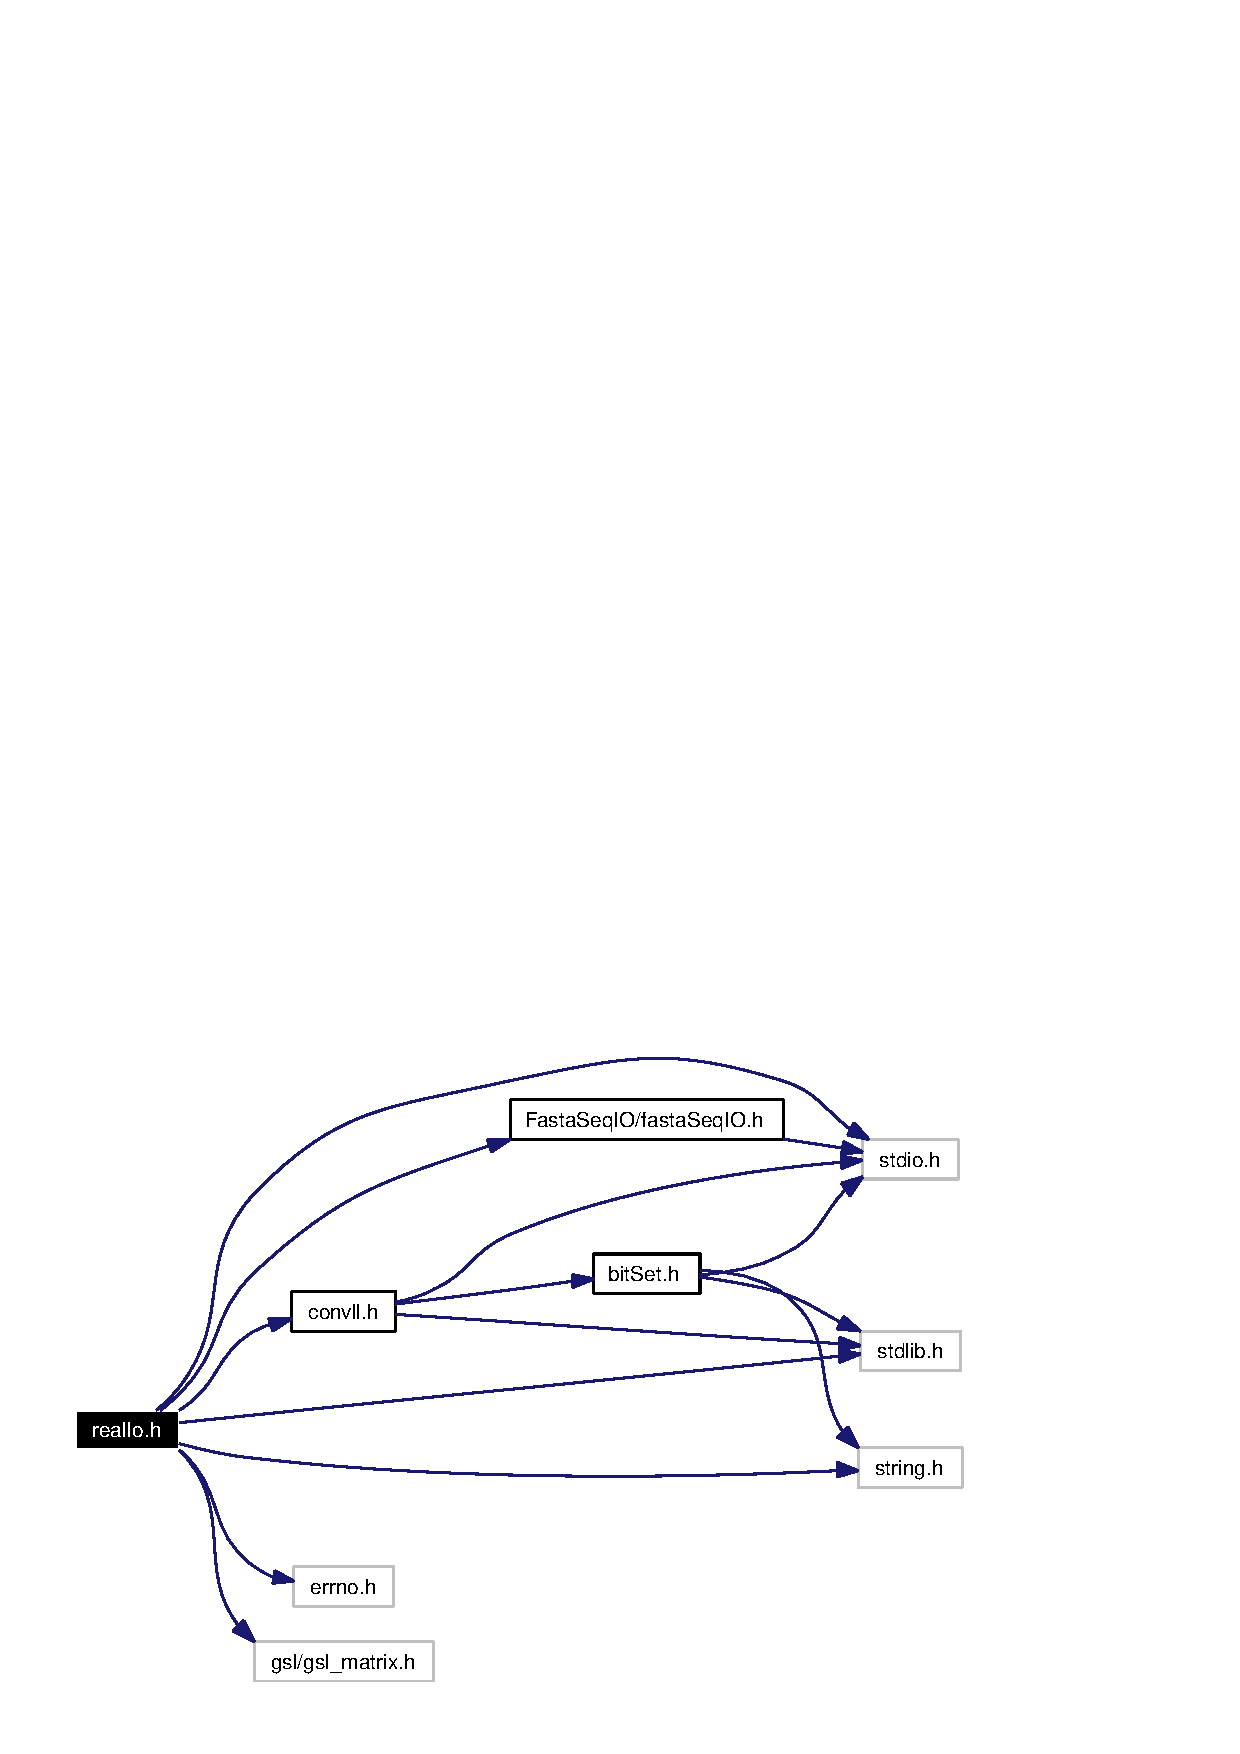
\includegraphics[width=231pt]{realIo_8h__incl}
\end{center}
\end{figure}


This graph shows which files directly or indirectly include this file:\begin{figure}[H]
\begin{center}
\leavevmode
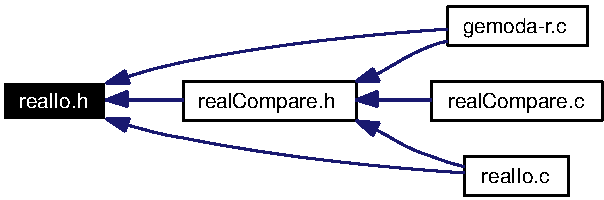
\includegraphics[width=162pt]{realIo_8h__dep__incl}
\end{center}
\end{figure}
\subsection*{Data Structures}
\begin{CompactItemize}
\item 
struct \hyperlink{structrdh__t}{rdh\_\-t}
\end{CompactItemize}
\subsection*{Functions}
\begin{CompactItemize}
\item 
\hyperlink{structrdh__t}{rdh\_\-t} $\ast$ \hyperlink{realIo_8h_a0}{read\-Real\-Data} (FILE $\ast$INPUT)
\item 
\hyperlink{structrdh__t}{rdh\_\-t} $\ast$ \hyperlink{realIo_8h_a1}{free\-Rdh} (\hyperlink{structrdh__t}{rdh\_\-t} $\ast$data)
\item 
int \hyperlink{realIo_8h_a2}{init\-Rdh\-Index} (\hyperlink{structrdh__t}{rdh\_\-t} $\ast$data, int word\-Size, int seq\-Gap)
\item 
int \hyperlink{realIo_8h_a3}{get\-Rdh\-Index\-Seq\-Pos} (\hyperlink{structrdh__t}{rdh\_\-t} $\ast$data, int index, int $\ast$seq, int $\ast$pos)
\item 
int \hyperlink{realIo_8h_a4}{get\-Rdh\-Dim} (\hyperlink{structrdh__t}{rdh\_\-t} $\ast$data)
\item 
int \hyperlink{realIo_8h_a5}{output\-Real\-Pats} (\hyperlink{structrdh__t}{rdh\_\-t} $\ast$data, \hyperlink{structcnode}{cll\_\-t} $\ast$all\-Pats, int L, FILE $\ast$OUTPUT\_\-FILE, int $\ast$$\ast$d)
\item 
int \hyperlink{realIo_8h_a6}{output\-Real\-Pats\-WCentroid} (\hyperlink{structrdh__t}{rdh\_\-t} $\ast$data, \hyperlink{structcnode}{cll\_\-t} $\ast$all\-Pats, int L, FILE $\ast$OUTPUT\_\-FILE, double $\ast$extra\-Params, int comp\-Func)
\end{CompactItemize}


\subsection*{Function Documentation}
\hypertarget{realIo_8h_a1}{
\index{realIo.h@{real\-Io.h}!freeRdh@{freeRdh}}
\index{freeRdh@{freeRdh}!realIo.h@{real\-Io.h}}
\subsubsection[freeRdh]{\setlength{\rightskip}{0pt plus 5cm}\hyperlink{structrdh__t}{rdh\_\-t}$\ast$ free\-Rdh (\hyperlink{structrdh__t}{rdh\_\-t} $\ast$ {\em data})}}
\label{realIo_8h_a1}


This function returns a null pointer after freeing the memory associated with a real data holder object. The function takes one parameter: a pointer to the real data holder, {\em data\/}.

Definition at line 396 of file real\-Io.c.

References rdh\_\-t::index\-To\-Pos, rdh\_\-t::index\-To\-Seq, rdh\_\-t::label, rdh\_\-t::offset\-To\-Index, rdh\_\-t::seq, and rdh\_\-t::size.

Referenced by main().



\hypertarget{realIo_8h_a4}{
\index{realIo.h@{real\-Io.h}!getRdhDim@{getRdhDim}}
\index{getRdhDim@{getRdhDim}!realIo.h@{real\-Io.h}}
\subsubsection[getRdhDim]{\setlength{\rightskip}{0pt plus 5cm}int get\-Rdh\-Dim (\hyperlink{structrdh__t}{rdh\_\-t} $\ast$ {\em data})}}
\label{realIo_8h_a4}


This function returns an integer equal to the dimensions of the data stored in a real data holder object. The function takes one parameter: a pointer to the real data holder, {\em data\/}.

Definition at line 447 of file real\-Io.c.

References rdh\_\-t::seq.

Referenced by general\-Match\-Factor(), get\-Rdh\-Value(), mass\-Spec\-Compare\-WElut(), print\-Rdh\-Seq(), rmsd\-Compare(), and set\-Rdh\-Value().



\hypertarget{realIo_8h_a3}{
\index{realIo.h@{real\-Io.h}!getRdhIndexSeqPos@{getRdhIndexSeqPos}}
\index{getRdhIndexSeqPos@{getRdhIndexSeqPos}!realIo.h@{real\-Io.h}}
\subsubsection[getRdhIndexSeqPos]{\setlength{\rightskip}{0pt plus 5cm}int get\-Rdh\-Index\-Seq\-Pos (\hyperlink{structrdh__t}{rdh\_\-t} $\ast$ {\em data}, int {\em index}, int $\ast$ {\em seq}, int $\ast$ {\em pos})}}
\label{realIo_8h_a3}


This function is used to access and change the sequence and position values, given an index. The function takes four parameters: a pointer to the real data holder, {\em data\/}, an integer {\em index\/}, a pointer integer {\em seq\/}, and a pointer integer {\em pos\/}.

Definition at line 544 of file real\-Io.c.

References rdh\_\-t::index\-Size, rdh\_\-t::index\-To\-Pos, and rdh\_\-t::index\-To\-Seq.

Referenced by general\-Match\-Factor(), make\-Alternate\-Centroid(), mass\-Spec\-Compare\-WElut(), output\-Real\-Pats(), output\-Real\-Pats\-WCentroid(), real\-Comparison(), and rmsd\-Compare().



\hypertarget{realIo_8h_a2}{
\index{realIo.h@{real\-Io.h}!initRdhIndex@{initRdhIndex}}
\index{initRdhIndex@{initRdhIndex}!realIo.h@{real\-Io.h}}
\subsubsection[initRdhIndex]{\setlength{\rightskip}{0pt plus 5cm}int init\-Rdh\-Index (\hyperlink{structrdh__t}{rdh\_\-t} $\ast$ {\em data}, int {\em word\-Size}, int {\em seq\-Gap})}}
\label{realIo_8h_a2}


This function is used to initialize the two indices inside a real data holder. The function takes as its input three parameters a pointer to the real data holder, {\em data\/}, the size of the words to be compared during the comparison stage {\em word\-Size\/}, and an integer {\em seq\-Gap\/}, which is used to place empty data between unique sequences, such that we do not convolve from one sequence into another during the convolution stage.

Definition at line 307 of file real\-Io.c.

References get\-Rdh\-Seq\-Length(), rdh\_\-t::index\-Size, rdh\_\-t::index\-To\-Pos, rdh\_\-t::index\-To\-Seq, rdh\_\-t::offset\-To\-Index, and rdh\_\-t::size.

Referenced by real\-Comparison().



\hypertarget{realIo_8h_a5}{
\index{realIo.h@{real\-Io.h}!outputRealPats@{outputRealPats}}
\index{outputRealPats@{outputRealPats}!realIo.h@{real\-Io.h}}
\subsubsection[outputRealPats]{\setlength{\rightskip}{0pt plus 5cm}int output\-Real\-Pats (\hyperlink{structrdh__t}{rdh\_\-t} $\ast$ {\em data}, \hyperlink{structcnode}{cll\_\-t} $\ast$ {\em all\-Pats}, int {\em L}, FILE $\ast$ {\em OUTPUT\_\-FILE}, int $\ast$$\ast$ {\em d})}}
\label{realIo_8h_a5}


This function is used to print out motifs discovered by Gemoda in an attractive fashion. The function takes five parameters: a pointer to a real data holder object {\em data\/}; a pointer to a linked list of motifs {\em all\-Pats\/}; an integer which is Gemoda's input parameter {\em L\/}; and a pointer to a file handle to which output is printed {\em OUTPUT\_\-FILE\/}.

Definition at line 904 of file real\-Io.c.

References get\-Rdh\-Index\-Seq\-Pos(), cnode::length, c\-Set\_\-t::members, cnode::next, rdh\_\-t::seq, cnode::set, c\-Set\_\-t::size, and cnode::stat.

Referenced by main().



\hypertarget{realIo_8h_a6}{
\index{realIo.h@{real\-Io.h}!outputRealPatsWCentroid@{outputRealPatsWCentroid}}
\index{outputRealPatsWCentroid@{outputRealPatsWCentroid}!realIo.h@{real\-Io.h}}
\subsubsection[outputRealPatsWCentroid]{\setlength{\rightskip}{0pt plus 5cm}int output\-Real\-Pats\-WCentroid (\hyperlink{structrdh__t}{rdh\_\-t} $\ast$ {\em data}, \hyperlink{structcnode}{cll\_\-t} $\ast$ {\em all\-Pats}, int {\em L}, FILE $\ast$ {\em OUTPUT\_\-FILE}, double $\ast$ {\em extra\-Params}, int {\em comp\-Func})}}
\label{realIo_8h_a6}


This function is used to output real valued patterns in a format such that they are centered on a particular centroid.

Definition at line 1068 of file real\-Io.c.

References find\-Clique\-Centroid(), get\-Comp\-Func, get\-Rdh\-Index\-Seq\-Pos(), cnode::length, make\-Alternate\-Centroid(), c\-Set\_\-t::members, cnode::next, cnode::set, and c\-Set\_\-t::size.

Referenced by main().



\hypertarget{realIo_8h_a0}{
\index{realIo.h@{real\-Io.h}!readRealData@{readRealData}}
\index{readRealData@{readRealData}!realIo.h@{real\-Io.h}}
\subsubsection[readRealData]{\setlength{\rightskip}{0pt plus 5cm}\hyperlink{structrdh__t}{rdh\_\-t}$\ast$ read\-Real\-Data (FILE $\ast$ {\em INPUT})}}
\label{realIo_8h_a0}


This function is used to read in a fasta formatted file containing real value data and store the entire thing and a real data holder object. The function takes one parameter: a pointer to a file handle, which is where the data are read from {\em INPUT\/};

Definition at line 850 of file real\-Io.c.

References check\-Real\-Data\-Format(), parse\-Real\-Data(), and Read\-File().

Referenced by main().



